In order to classify dark spots as either oil spills or lookalikes, features are extracted from them to calculate the probability for the two possible outcomes. A feature is an identified measurable property concerning the dark spot and which value has a strong statistical relationship with the classification output. Around 25 features are commonly used for oil spill classification and can be found in \ref{fig:featuretable}.

\begin{figure}[H]
	\centering
    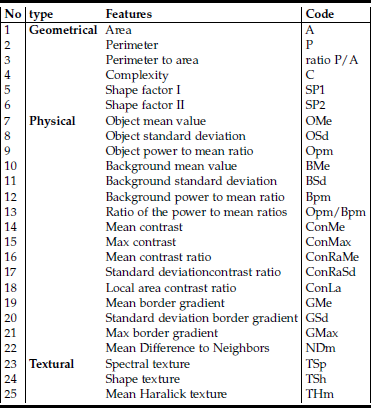
\includegraphics[width=0.4\textwidth]{./img/featurestable.png}
    \caption{\footnotesize{The 25 most commonly used features\cite{Topouzelis201268}}}
    \label{fig:featuretable}
\end{figure}

The features can be divided into three major categories\cite{Brekke200595}:
\begin{enumerate}
\item (1 - 6) geometric characteristics (e.g. area, perimeter, complexity)
\item (7 - 22)Physical characteristics of the backscatter level of the spot and its surroundings (e.g. mean, max backscatter value)
\item (23 - 25) Texture (e.g. mean contrast)
\end{enumerate}

Geometric characteristics are the features that are related to the shape of the dark spot and is applied by all methods in the table \cite{Topouzelis200930}. An important feature is how elongated a spot is, which is expressed as a ratio between the width and length of the dark spot \cite{Gasull20071}. A study has shown that oil spills can be discriminated according to their shape \cite{Guo2014146}. The majority of oil spills have a linear shape that is either straight or angular \cite{Pavlakis200156}. Features that use the backscatter level of the spot and its surroundings take into account the gradient level in the image. For example, the background standard deviation is a feature that is highly effected by wind level and is generally high for lookalikes. Texture provides information about the spatial correlation among neighbouring pixels. Contextual features are not included in the table, but are considered very useful \cite{Topouzelis200930}. They incorporate other information not all extractable from the image, but is available as prior knowledge. These include the distance between a dark spot and a ship, weather information, distance to shore and whether the dark spot lies in a frequently polluted area. Most classifiers rely heavily on geometric shape features and the contextual feature. \cite{Xu201414}

Researchers try to reduce the amount of features to counter the curse of dimensionality which makes the dataset become more sparse as the dimensionality increases. Training a classifier with a sparse dataset will have lower predictive power. Fewer features also reduce the risk of over fitting, which is what happens when the classifier is too trained on specific data instead of capturing the underlying relationship. This leads to poor generalization of the data and thus has an negative impact on the classification process.

Features belonging to the same category appear to be highly correlated \cite{Xu201414}, leading to the search for a subset of features with less redundancy and retains most of the predictive power. How many and which features to include is known as the feature selection problem. Including too many features leads to a larger geometric space requiring the classifier to be more complex. Important information is lost when leaving too many features out, researchers try to find the right balance. The resulting subset will allow shorter training times and reduce over fitting. The values of these features are calculated and used as inputs in a chosen classifier.
